\documentclass[14pt]{extreport}
\usepackage[utf8]{inputenc}
\usepackage[english,russian]{babel}

\usepackage{array}
\usepackage{setspace}
\usepackage[pdftex]{graphicx}
\usepackage{graphicx}
\graphicspath{{img/}}
\usepackage{subcaption}


\usepackage{algorithm}
\usepackage{algpseudocode}

\usepackage[nottoc,numbib]{tocbibind} %bibliography in table of contents

\usepackage{titlesec} % decrease chapter heading sizes
    \titleformat{\chapter}[display]
      {\normalfont\large\bfseries\filcenter}{\chaptertitlename\ \thechapter}{0pt}{\Large} %huge 10 Huge
    \titlespacing*{\chapter}
      {0pt}{0pt}{10pt} %10 30 20 default

\makeatletter
\renewcommand{\@biblabel}[1]{#1.} % Заменяем библиографию с квадратных скобок на точку:
\renewcommand{\baselinestretch}{1.5}
\makeatother

\usepackage[left=3.0cm,right=1.5cm,top=2.0cm,bottom=2.0cm,bindingoffset=0cm]{geometry}

\begin{document}

   \begin{titlepage}{
        \thispagestyle{empty}\newgeometry{left=2.5cm,right=1.5cm,top=0cm,bottom=0.2cm,bindingoffset=0cm}\setstretch{1}
        \begin{center}
            {\footnotesize
                Министерство образования и науки Российской Федерации\\
                Федеральное государственное автономное образовательное учреждение\\
                высшего профессионального образования\\
            }

            <<Уральский федеральный университет\\
             имени первого Президента России Б.Н.Ельцина>>

             \vskip+0.5cm

            Институт математики и компьютерный наук\\
            Кафедра вычислительной математики

            \vskip+25mm

            {\bf \LARGE
                Поиск вредоносной активности в DNS трафике \\
            }

            \vskip+15mm
        \end{center}
	
        \vfill
        \noindent\begin{parbox}[t]{9cm}{\small
                \vspace{2.0cm}
                Допустить к защите:

                \bigskip
                \bigskip
                \bigskip

                \hbox to45mm{\hrulefill}

                \bigskip

                <<\,\hbox to10mm{\hrulefill}\,>>  \hbox to25mm{\hrulefill}  2016 г.
            }
            \end{parbox}
            \begin{parbox}[t]{9cm}{\small  \setstretch{1}
                Выпускная квалификационная работа \\
                на степень бакалавра по направлению\\
                02.03.02
                Фундаментальная информатика \\
                и информационные технологии	 \\
                студента группы МК-420002 \\
                                \bigskip
                Меньших Ивана Александровича\\
                Научный руководитель\\
                доцент Солодушкин Святослав Игоревич\\
            }
            \end{parbox}
        \vfill
        \centerline{Екатеринбург}
        \centerline{2016}
        }\restoregeometry
    \end{titlepage}
\newpage
    \tableofcontents

\newpage
    \chapter{Введение в проблему поиска вредоносной активности}

Важнейшей задачей, стоящей перед системными администраторами, является защита корпоративной сети и пресечение любых вредоносных взаимодействий клиентов сети и сети интернет. Схожая задача стоит перед сервисами, предоставляющими услуги DNS фильтрации. Анализ логов DNS сервера позволяет выделить в общей массе запросов <<подозрительные>> (т.е. те, которые соответствуют коммуникации зараженного хоста и, например, управляющего C\&C сервера). 

В реальности, анализ DNS логов проводить крайне трудно, потому что каждый клиент генерирует большое количество запросов. Даже при заходе на сайт пользователь генерирует множество запросов. Как правило, при загрузке страницы происходят обращения на сторонние сервера для загрузки стилей, скриптов, изображений и так далее. Даже когда пользователь ничего не делает, его ПК генерирует запросы. Это могут быть обновления программного обеспечения, синхронизация часов и так далее. Особенно это заметно в новых версиях Windows: операционная система старается <<радовать>> пользователя своей интерактивностью и постоянно запрашивает новости, курсы валют, отправляет различную информацию о его действиях на свои сервера для <<персонализации>> взаимодействия.

В этой работе будут рассмотрены различные способы анализа DNS трафика, на базе которых можно выделить домены, которые, вероятно, используются для коммуникации между зараженным хостом и ботмастером.

\newpage
Общая идея заключается в анализе паттернов взаимодействия зараженных клиентов и C\&C серверов. Кроме того, речь будет идти о фильтрации запросов. Это очень важный аспект, ведь известно, что <<Garbage In, Garbage Out>>. Будут сделаны несколько предположений о структуре паттернов взаимодействия, а также предложены методы анализа.

\chapter{Формальная постановка задачи}
	Для того, чтобы приступить к решению этой проблемы, необходимо формализовать задачу.
	
	{\bfДано:}
		
		1. DNS логи ($querylog$). Определим их как множество $Q$. Каждая запись в нём представима в виде вектора признаков $\vec{query}$$\in$$Q$, который \textbf{обязательно} содержит $source\_ip$ (ip адрес клиента, который совершает запрос) и $domain$ (домен, который пользователь желает <<разрешить>>). Кроме того, в нём могут содержаться дополнительные данные (например время, когда был совершен запрос, подробно структура $\vec{query}$ будет описана далее).
		
		2. Белый список доменов ($whitelist$). Будем использовать <<самые частопосещаемые>> домены, для этого воспользуемся списками от Alexa и Quantcast)
		
		3. Черный список доменов ($blacklist$). Будем использовать базы компании SkyDNS и прочие источники.
	
	{\bfНеобходимо:} 
	
	1. Выбрать из $querylog$ подмножество 
	запросов $\{\vec{query_1}, \vec{query_2}, \vec{query_3}, \dots\}$, которые были совершены к вредоносным доменам и выделить имена этих доменов. На самом деле, нас больше интересуют сами доменные имена, так как по ним легко осуществлять блокировку	(что и является основной нашей задачей)
	
	2. Выделить общие паттерны взаимодействия клиентов и вредоносных доменов, описать внешний вид графа запросов.
	
	\section{Структура $\vec{query}$}
		\begin{tabular}{| l | r |}
			\hline
			Поле & Описание \\ \hline
			$domain$ & Домен, который был запрошен пользователем \\ \hline 
			$source\_ip$ &  IP адрес пользователя \\ \hline
			$rcode$ &  Код возврата DNS сервера \\ \hline
			$qtype$ &  Код запрашиваемого типа записи \\ \hline
			$timestamp$ &  Временная метка получения сервером запроса \\ \hline

		\end{tabular}
		
	
	\section{Структура $whitelist$ и $blacklist$}
	\begin{tabular}{| l | r |}
			\hline
			Поле & Описание \\ \hline
			$domain$ & Доменное имя \\ \hline 
			$cats$ & Cписок категорий, к которым принадлежит домен \\ \hline

	\end{tabular}
	\section{Словарь}
	\begin{tabular}{p{3cm} p{10cm}}
	\hline
			Домен & Символьное имя, служащее для идентификации областей — единиц административной автономии в сети Интернет — в составе вышестоящей по иерархии такой области. \\ 
			TLD & Домен верхнего (первого) уровня (например .com, .eu) \\
			iLD & Домен i уровня \\
			Хост & Клиентский ПК \\
			Ботнет & Сеть из заражённых хостов, управляемая ботмастером через C\&C сервер \\
			C\&C & Управляющий сервер ботнета \\
			 \hline

	\end{tabular}
	
	\chapter{Ботнеты}
	\section{Описание}
	Ботнет - сеть инфицированных хостов, управляемая извне. Бот, по своей сути, это вредоносное программное обеспечение, которое позволяет злоумышленнику удаленно управлять устройством пользователя.
	
	Заражение подобным программным обеспечением может происходить через
уязвимости в используемом ПО (например через браузер и эксплуатации 0-day
exploit, который позволяет исполнить произвольный код за пределами
«песочницы» браузера). Кроме того, заражение может произойти с помощью
«социальная инженерии», где вредоносное ПО маскируется под полезное
содержимое, например вложение в электронном письме.

	Проблема детектирования ботнетов стоит очень остро, так как они растут вместе с интернетом. Например один из самых больших - ботнет Ponmocup, по данным компании FoxIT, достигал размера 15000000 хостов.
	
	Очень важно научиться выявлять ботнеты, а именно, в рамках текущей
работы, нас интересуют доменные имена, которые используют C\&C сервера.
Это поможет нам предупредить пользователей, чьи ПК проявляют
«аномальную» активность, схожую с активностью члена ботнета.
	
	\newpage
	\section{Топология}
	Можно выделить две основных топологии построения ботнетов \cite{communication}
	

	\begin{figure}[H]
	
	\begin{subfigure}{0.5\textwidth}
	\includegraphics[width=0.9\linewidth, height=5cm]{star_topology.png}
	\caption{<<Звезда>>}
	\label{fig:subim1}
	\end{subfigure}
	\begin{subfigure}{0.5\textwidth}
	\includegraphics[width=0.9\linewidth, height=5cm]{tree_topology.png}
	\caption{<<Дерево>>}
	\label{fig:subim2}
	\end{subfigure}
	 
	\caption{Популярные варианты топологии ботнета}
	\label{fig:image2}
	\end{figure}
	Топология, изображённая на Рис. 3.1.(a) является, пожалуй, самой часто встречающейся и простой. Зараженные хосты напрямую коммуницируют с C\&C сервером. Основная её уязвимость - централизация. Благодаря этому аспекту, отследить управляющий сервер гораздо проще. Соответственно, и обезвредить такой ботнет легче. Из плюсов стоит отметить быструю коммуникацию, т.к. отсутствует <<прослойка>> между клиентом и сервером.
	Как расширение данной топологии, можно рассматривать вариант, в котором используется несколько серверов. Это убирает проблему с единой точкой отказа, а также позволяет балансировать нагрузку по географической принадлежности (для общения с хостом используется сервер, который к нему физически ближе). Минус - дополнительные затраты на сервера, а также сложность в синхронизации между серверами.
	
	Топология из Рис. 3.1.(b) встречается реже, но является более устойчивой. Смысл заключается в том, что зараженные хосты общаются с управляющим сервером через <<прокси>>, в качестве которого выступают другие зараженные хосты. Это позволяет скрыть реальный C\&C сервер, что препятствует его обнаружению. Кроме того, ботнет проще будет <<продать>> по частям, продавая контроль над некоторым поддеревом данного графа (а дерево может быть достаточно глубоким).
	
	Также встречается топология вида P2P, где хосты соединены между собой и образуют небольшие плотные графы. Это самый устойчивый вариант, но им сложно управлять. В нём просто нет места для C\&C сервера и команды, фактически, передаются какому-либо хосту, который распространяет эту команду всем остальным.

	
	\newpage
	\section{Стратегии уклонения}
	Для того, чтобы предотвратить обнаружение управляющий серверов и уничтожение ботнета, ботмастеры используют различные стратегии, препятствующие этому \cite{communication}.
	\subsection{IP Flux (fast flux)}
	Один из вариантов - использовать много ip адресов для одного доменного имени и маленький TTL для A записи в DNS пакете. Данный приём можно усложнить, меняя также ip адреса соответствующий NS серверов.
	
	Изначально, данный приём позволял легитимными сайтами балансировать нагрузку между серверами еще на этапе разрешения доменного имени. Этот способ до сих пор используется разными сайтами (например google.com)
	
	\subsection{Domain Flux}
	Другой вариант - использовать много доменных имён, разрешающихся в один ip адрес. Именно этот подход чаще всего используется в настоящее время. Связано это с исчерпанием IPv4 диапазона. В это же время, доменное имя практически ничего не стоит. Кроме того, владея 2LD доменом, можно легко генерировать множество 3LD доменов (example.com -> *.example.com) .
	Как правило, для этого используются специальные алгоритмы, которые генерируют домены на основе системного времени. Класс таких доменов называется DGA. Они являются короткоживущими (несколько часов - несколько недель) и используются для одноразовой коммуникации. 
	
   \section{Коммуникация}
   \begin{figure}[H]
   	\centering
	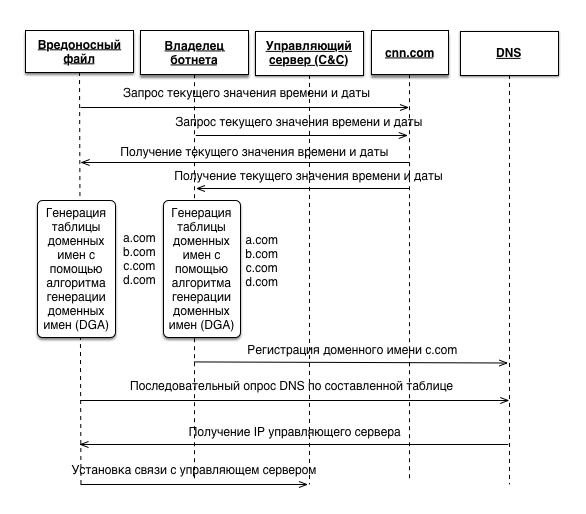
\includegraphics[scale=0.8]{communicate.png}
	\caption{Принцип работы}
	\end{figure}
	Процесс коммуникации можно разделить на несколько шагов, они изображены на Рис. 3.2. Опишем подробней эту схему:
	
	1. Заражённый хост и управляющий сервер синхронизируют время путём отправки запроса по протоколу NTP к некоторому серверу точного времени. Эта стадия происходит не всегда, если не требуется синхронизации по минутам/секундам. Зачастую, хватает точности до суток.
	
	2. Хост и C\&C сервер генерируют доменные имена, основываясь на текущей временной метке.
	
	3. C\&C сервер регистрирует эти доменные имена
	
	4. Клиент опрашивает сгенерированные доменные имена по списку и пытается получить ip адрес
	
	5. Клиент устанавливает соединение с C\&C сервером и получает необходимые команды/обновления
	
Таким образом, теперь мы имеем базовое представление о ботнетах, их структуре и поведении.

	\chapter{Групповая активность}
	\section{Описание}
	Один из подходов поиска ботнетов - отслеживание групповой активности клиент-домен. Основываясь на работе \cite{groupact} сделаем несколько предположений:
	
	1. Заражённых хостов в сети фиксированное количество
	
	2. Взаимодействие заражённых хостов и C\&C сервера проявляется переодически
	
	3. Как правило, используется техника domain flux, которая была описана выше (используется много доменных имён и мало ip адресов)
	
	Исходя из данных предположений, можно составить алгоритм, который выделит подозрительные коммуникации между группами хостов и доменом.
	
	\section{Алгоритм}
	
	Алгоритм поиска групповой активности можно разделить на 3 стадии: сбор информации о запросах пользователей, фильтрация запросов и детектирование подозрительной активности. 
	
	Изначально, мы делим все $querylog$ на <<окна>>, в текущем случае использовалось окно длины 1 час. Выбрано это число из таких соображений: частая коммуникация не свойственна ботнетам, поэтому не имеет смысл использовать окно меньшего размера. Кроме того, при слишком маленьком окне, высок шанс ложного срабатывания алгоритма, а при слишком большом - слабой чувствительности.
	
	Первая функция группирует все пары запросов ($client\_ip$, $domain$) по домену. Подобная агрегация позволяет получить представление о том, кто именно запрашивает конкретный домен.
	\begin{algorithmic}
	\Function{SearchInfo}{$querylog$ [by hour]}
	\State $data\gets Dictionary<str, set>$
	\For{($client\_ip$, $domain$) in $querylog$} 
	
		\State $data[domain]$.add($client$)
	\EndFor
	
	\State \Return $data$
	\EndFunction
	\end{algorithmic}

	Следующая функция фильтрует полученные данные. Нам необходимо исключить все доменные имена, которые есть в $whitelist$, а также те доменные имена, которые запрашиваются малым количеством пользователей (хорошим вариантом будет значение $threshould$ $\in$ 3, 4, 5, 6, 7)
	

	\begin{algorithmic}
	\Function{FilterQueries}{$data<str,set>$, $whitelist$, $threshould$}
	\For{$domain$ in $data$}
		\If{$domain$ in $whitelist$ OR length(data[domain]) < threshould}
			\State $ip\_list\gets data[domain]$
			\State $data$.remove($domain$)
			\State $data$.pop\_values($ip\_list$)
		\EndIf
		
		
	\EndFor
	\State \Return $data$
	\EndFunction
	\end{algorithmic}
	
	Последняя функция выполняет предварительную обработку $querylogs$, выбирает доменные имена, к которым в разные временные промежутки обращаются, в основном, одни и те же пользователи, что, в рамках наших начальных предположений, говорит о вредоносности такого домена
	\begin{algorithmic}
	\Function{DetectBotnetDomain}{$querylogs<list>$, $sim\_score$}
	\State $data\_arr\gets List<dictionary>$
	\State $botnet\_domains\gets Set<str>$
	\For{$querylog$ in $querylogs$}
		\State $curr\_data\gets SearchInfo(querylog)$
		\State $curr\_data\gets FilterQueries(curr\_data)$
		\State $data\_arr$.append($curr\_data$)

	\EndFor
	\For{$data_1$ in $data\_arr$}
		\For{$data_2$ in $data\_arr$}
			\If{$data_1$ $\ne$ $data_2$}
				\For{$domain$ in $data_1$ $\cap$ $data_2$}
					\State $curr\_sim\gets Similarity(data_1[domain], data_2[domain])$
					\If{$curr\_sim$ > $sim\_score$}
						\State $botnet\_domains$.add($domain$)
					\EndIf
				\EndFor
			\EndIf
		\EndFor
	\EndFor
	\State \Return $botnet\_domains$
	\EndFunction
	\end{algorithmic}
	
	
	Немного о функции $similarity$, она выражает <<схожесть>> между клиентами, которые запрашивают один и тот же домен. В работе [2] предлагается для этих целей использовать такую функцию: 
	$$similarity(ipList_1, ipList_2) = \frac{1}{2} * (\frac{C}{A} + \frac{C}{B}) (A\ne0, B\ne0)$$
	где $A = |ipList_1|$, $B = |ipList_2|$, $C = |ipList_1\cap ipList_2|$
	
	Эксперименты показали, что есть более подходящая функция - расстояние Джаккара: $$similarity(iplist_1, iplist_2) = \frac{|ipList_1\cap ipList_2|}{|ipList_1\cup ipList_2|}$$
	
	Таким образом, мы рассмотрели вариант детектирования подозрительных доменных имен, основанный на групповой активности.
	
	\chapter{Ранжирование доменов}
	Это я пробую сейчас, пока получаются странные результаты, которые я не могу объяснить, требует сборки тестового стенда
	\section{Описание подхода}
	тут будет текст
	\section{Алгоритм}
	тут будет текст

	\chapter{<<Графовый>> подход}
	Это я начал делать, упёрся в три-факторизацию матриц, буду продолжать как закончу предыдущие. Но именно этот подход выглядит как самый перспективный
	\section{Описание подхода}
	тут будет текст
	\section{Алгоритм}
	

	
	%\chapter{Анализ временных рядов запросов}
	%Попробовал, после преобразования Фурье получаю очень много шума, нужно придумать как чистить
	%\section{Описание подхода}
	%тут будет текст
	%\section{Алгоритм}
	%тут будет текст
	
	%\chapter{Байесовский подход}
	%Ещё не пробовал, ничего сказать пока не могу. Возможно не успею сделать и выброшу его совсем из диплома.
	%\section{Описание подхода}
	%тут будет текст
	%\section{Алгоритм}
	%тут будет текст

	\chapter{Результаты исследований}
	тут будет текст %\cite{doe:website}
	
\addcontentsline{toc}{chapter}{Литература}
\begin{thebibliography}{99}

\bibitem{communication} Gunter Ollmann, ``Botnet Communication Topologies. Understanding the intricacies of botnet command-and-control'', 2009.

\bibitem{groupact} Hyunsang Choi, Hanwoo Lee, Heejo Lee, Hyogon Kim, ``Botnet Detection by Monitoring Group Activities in
DNS Traffic''.

\end{thebibliography}

%\addcontentsline{toc}{chapter}{bibname}
%\bibliographystyle{utf8gost705u}
%\bibliography{biblio}
\end{document} 